\documentclass{article}
\usepackage[french]{babel}
\usepackage[T1]{fontenc}
\usepackage{import}
\usepackage{hyperref}
\usepackage{graphicx}


\title{Être et Avoir}
\author{Lucas Santiago de Oliveira}
\date{Mars, 2022}

\begin{document}
    \maketitle

    \vspace{2cm}

    \href{https://www.youtube.com/watch?v=Z2hZIJFg9v4}{Le lien de la vidéo}
    
    \includegraphics[angle=270, width=\textwidth]{images/etre et avoir stucturaux.jpg}
    \newpage

    \begin{center}
        \section*{Être et Avoir}
        \begin{tabular}{|c|c|c|}
            \hline
            Pronoms Sujets & Être & Avoir \\
            \hline
            je & suis & j'ai \\
            \hline
            tu & es & as \\ 
            \hline
            il / elle / on & est & a \\
            \hline
            nous & sommes & avons \\
            \hline
            vous & être & avez \\
            \hline
            ils / elles & sont & ont \\
            \hline
        \end{tabular}
    \end{center}

    \section*{Exercice 1}
    \import{exercices/exercise1}{exercise.tex}

    \newpage
    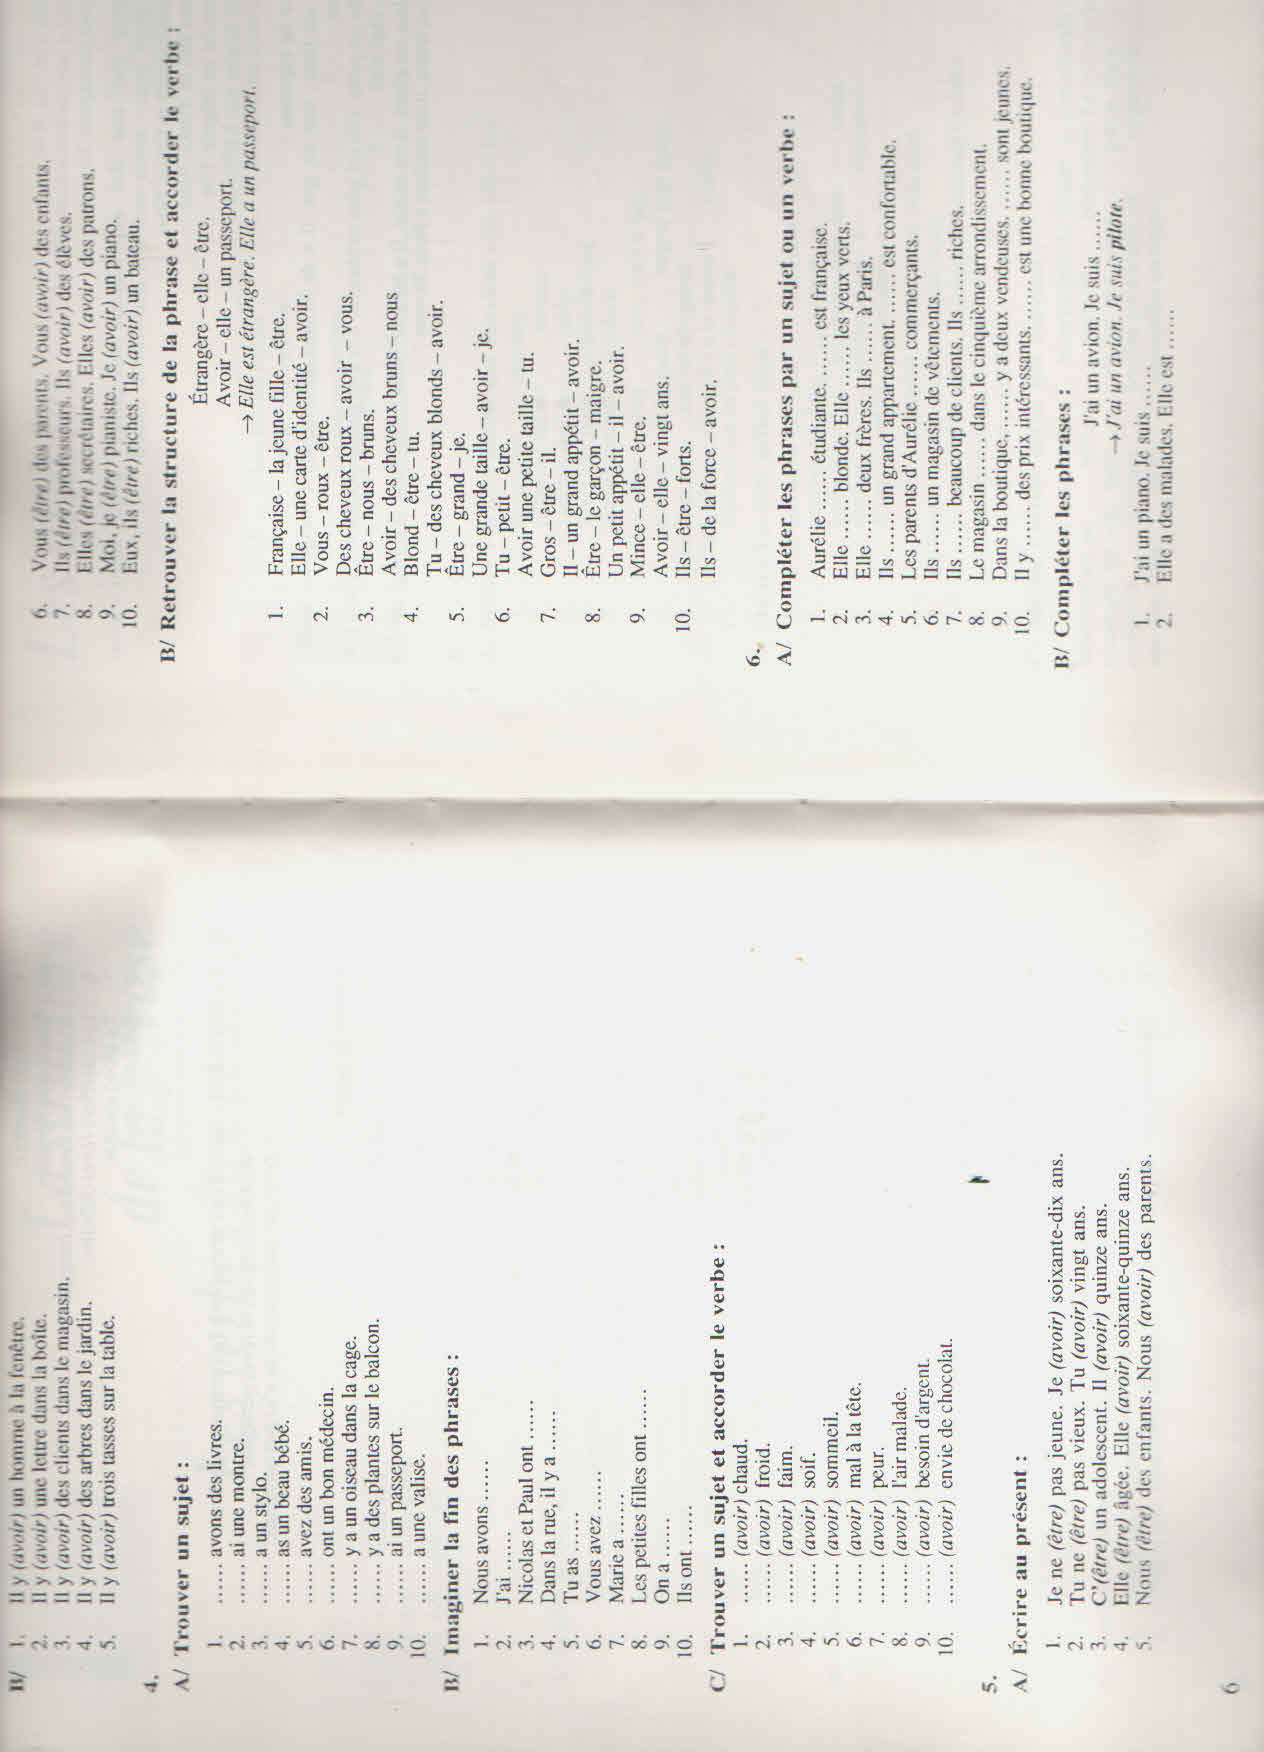
\includegraphics[angle=270, width=\textwidth]{images/etre et avoir stucturaux1.jpg}

    \section*{Exercise 2}
    \import{exercices/exercise2}{exercise.tex}

    \newpage
    \includegraphics[width=\textwidth]{images/etre et avoir stucturaux2.jpg}

    \section*{Exercise 3}
    \import{exercices/exercise3}{exercise.tex}
\end{document}